\documentclass[conference]{IEEEtran}
\usepackage[utf8]{inputenc}
\usepackage[T1]{fontenc}
\usepackage[spanish,es-nodecimaldot,es-tabla]{babel}
\addto\captionsspanish{\renewcommand{\figurename}{Fig.}}
\usepackage{amsmath}
\usepackage{graphicx}
\usepackage{booktabs}
\usepackage{url}
\usepackage{cite}

% Marca para lo que falta completar con tus datos reales
\newcommand{\pend}[1]{\textbf{[PENDIENTE: #1]}}

\begin{document}

\title{Laboratorio 1\\Estructura de datos}

\author{\IEEEauthorblockN{Iván Eduardo Rivas Guzmán}
\IEEEauthorblockA{Departamento de Ciencia de Datos\\
Universidad del Norte, Barranquilla, Colombia\\
ierivas@uninorte.edu.co}}

\maketitle

\begin{abstract}
Los videojuegos registran cada evento de la partida en bitácoras que crecen más rápido de lo que conviene cargar en memoria. Este trabajo presenta un sistema de telemetría para un videojuego en Pygame: un formato de línea delimitada, escritura incremental con buffer y rotación por tamaño, y un lector en streaming tolerante a líneas corruptas. Sobre ese lector se implementó, desde cero, un motor estadístico que calcula medidas descriptivas, cuartiles, atípicos, frecuencias, histograma, embudo de niveles y correlación, cuyos resultados se muestran dentro del juego. Los experimentos con hasta 100 000 eventos muestran que un buffer de 100 líneas aprovecha la mayor parte de la ganancia y que la lectura perezosa mantiene la memoria casi constante, frente a una carga completa que crece con el archivo.
\end{abstract}

\begin{IEEEkeywords}
telemetría, videojuegos, procesamiento en streaming, estadística descriptiva, Pygame
\end{IEEEkeywords}

\section{Introducción}
Los videojuegos modernos registran en una bitácora de eventos todo lo que ocurre en la partida: enemigos eliminados, daño recibido, muertes y niveles superados. Esos registros permiten responder preguntas de diseño, como en qué nivel abandonan los jugadores o si la dificultad está equilibrada \cite{drachen}. El problema es que la bitácora crece rápido: cargarla completa en memoria no escala, así que debe procesarse recorriéndola una sola vez y acumulando resultados.

El objetivo de este trabajo es construir ese sistema para un juego propio en Pygame: la escritura de la bitácora durante la partida, su lectura robusta desde archivos y un motor estadístico escrito desde cero, sin librerías estadísticas, cuyos resultados se dibujan dentro del propio juego.

\section{Diseño del sistema}
\subsection{Formato de la bitácora}
Cada evento ocupa una línea de texto con exactamente cuatro campos separados por \texttt{|}: \texttt{timestamp|sesion|evento|clave=valor;...}. Se eligió texto y no binario porque es legible sin herramientas, se escribe al final del archivo sin reorganizar nada y un daño queda confinado a una línea: si el juego se cierra de golpe, solo se pierde la última línea incompleta. En un formato binario de registros, un byte dañado puede desalinear todo lo que sigue. A cambio, el texto ocupa más espacio y obliga a convertir los números al leer.

Si un valor contuviera el delimitador, la línea tendría más de cuatro campos (o un parámetro mal formado) y se contaría como corrupta. En el juego esto se evita porque el nombre del jugador solo admite letras y números. Una solución general sería escapar los delimitadores, y eso no se implementó.

\subsection{Escritura}
El escritor abre el archivo en modo \emph{append} y acumula las líneas en un buffer de $N$ líneas, que vuelca con \texttt{flush()} al llenarse y al cerrar el juego. Cuando el archivo activo supera 512~KiB se cierra y se abre el siguiente (\texttt{events\_002.log}, etc.). El valor $N=100$ se justifica con el Experimento A (Sección~\ref{sec:disc}).

\subsection{Lectura, líneas corruptas y sesiones incompletas}
El lector es un generador que recorre los archivos en orden y entrega un evento a la vez con \texttt{for linea in f}, sin cargar el archivo. Una línea es corrupta si está vacía, no termina en salto de línea (truncada), no tiene cuatro campos, tiene un parámetro sin \texttt{=} o con valor vacío, o un valor numérico no convertible. Esas líneas se cuentan y se descartan sin detener el programa. Una carpeta inexistente o vacía produce cero eventos.

Una sesión sin \texttt{SESSION\_END} se reporta como incompleta. \textbf{Decisión:} no entra en las medidas por sesión (puntaje, duración, nivel, dificultad y correlación), porque sin el cierre esos valores se desconocen y usar valores parciales sesgaría los resultados a la baja. En cambio, sus eventos individuales (daño, causa de muerte) sí se cuentan, porque cada uno es una medición válida por sí sola.

\section{Metodología estadística}
Todas las medidas se implementaron desde cero. Las medidas descriptivas se calculan en un solo recorrido, acumulando $n$, $\sum x$, $\sum x^2$, el mínimo y el máximo:
\begin{equation}
\bar{x}=\frac{\sum x}{n}
\end{equation}
\begin{equation}
s^2=\frac{\sum x^2-n\bar{x}^2}{n-1},\qquad s=\sqrt{s^2}
\end{equation}
\begin{equation}
CV=\frac{s}{\bar{x}}\times 100\%
\end{equation}
La varianza muestral divide entre $n-1$ porque la media se estimó con los mismos datos.

Para los cuartiles se ordena la lista, se parte en una mitad inferior y otra superior (excluyendo la mediana central cuando $n$ es impar) y $Q_1$ y $Q_3$ son las medianas de cada mitad. El percentil 90 usa el rango más cercano: el dato en la posición $\lceil 0.9\,n\rceil$. Existen varias convenciones \cite{hyndman}, y esta reproduce los valores de referencia ($Q_1=1500$, $Q_3=3000$, $P_{90}=3600$). Los valores atípicos se detectan con la regla de Tukey \cite{tukey} y con el puntaje $z$:
\begin{equation}
[\,Q_1-1.5\,IQR,\;\; Q_3+1.5\,IQR\,],\quad IQR=Q_3-Q_1
\end{equation}
\begin{equation}
z=\frac{x-\bar{x}}{s},\qquad \text{atípico si } |z|>3
\end{equation}
La correlación de Pearson también se calcula en una pasada, acumulando $n$, $\sum x$, $\sum y$, $\sum xy$, $\sum x^2$ y $\sum y^2$:
\begin{equation}
r=\frac{n\sum xy-\sum x\sum y}{\sqrt{\left(n\sum x^2-(\sum x)^2\right)\left(n\sum y^2-(\sum y)^2\right)}}
\end{equation}
Para el embudo de niveles, con $N_k$ las sesiones que alcanzaron el nivel $k$, la supervivencia se mide contra el total y el abandono contra el nivel anterior:
\begin{equation}
S_k=\frac{N_k}{N_1}\times 100\%,\qquad A_k=\frac{N_{k-1}-N_k}{N_{k-1}}\times 100\%
\end{equation}
El histograma usa $k=8$ intervalos de ancho $w=(\max-\min)/8$. La Tabla~\ref{tab:memoria} resume qué estadísticas se calculan en una sola pasada y cuáles obligan a guardar los datos.

\begin{table}[t]
\caption{Estadísticas: una pasada y memoria}
\label{tab:memoria}
\centering
\footnotesize
\begin{tabular}{p{1.8cm}p{1.0cm}p{0.9cm}p{3.0cm}}
\toprule
Estadística & ¿Una pasada? & Memoria & Por qué \\
\midrule
media, mín., máx. & Sí & $O(1)$ & basta acumular $n$, suma, mínimo y máximo \\
varianza, desv., CV & Sí & $O(1)$ & se obtienen de $n$, $\sum x$ y $\sum x^2$ (3 acumuladores) \\
Pearson & Sí & $O(1)$ & 6 acumuladores \\
tabla de frecuencias & Sí & $O(c)$ & un contador por categoría distinta ($c$) \\
histograma de $k$ intervalos & No (2 pasadas) & $O(k)$ & el ancho exige conocer el mínimo y el máximo antes \\
mediana, cuartiles, P90 & No & $O(n)$ & hay que ordenar todos los datos \\
\bottomrule
\end{tabular}
\end{table}

\section{Metodología experimental}
Un generador de bitácoras sintéticas simula sesiones con los seis tipos de evento, con semilla fija, y se detiene exactamente en $5\,000$, $50\,000$ y $100\,000$ eventos. Se midió: (A) el tiempo de escribir $100\,000$ eventos con buffer de 1, 10, 100 y 1000 líneas, como promedio de tres corridas; (B) el tiempo de lectura, los eventos por segundo y los microsegundos por línea; y (C) el pico de memoria de la lectura perezosa frente a cargar todos los eventos en una lista. Los tiempos se midieron con \texttt{time.perf\_counter()} y la memoria con \texttt{tracemalloc} \cite{tracemalloc}, que se ejecutó aparte para no distorsionar los tiempos.

Equipo: procesador AMD Ryzen 7 5800X, 24~GB de RAM DDR4 a 2666~MT/s (3 módulos de 8~GB), disco duro mecánico (HDD), Windows 11 Pro, Python 3.14.8 y pygame-ce 2.5.8.

\section{Resultados}
\begin{figure}[t]
\centering
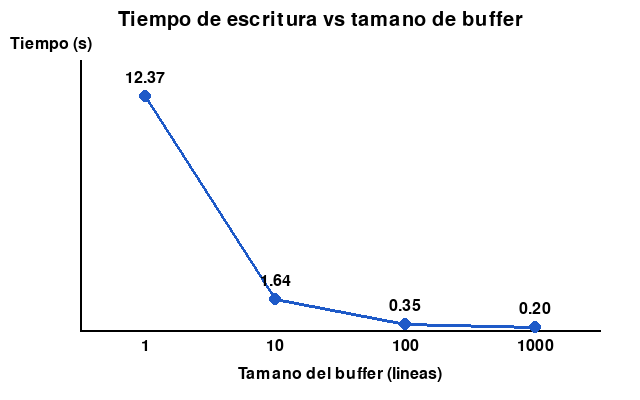
\includegraphics[width=\columnwidth]{resultados/figura_A.png}
\caption{Experimento A: tiempo de escritura de $100\,000$ eventos contra el tamaño del buffer.}
\label{fig:A}
\end{figure}

La Fig.~\ref{fig:A} muestra el Experimento A: 12.37~s con buffer de 1 línea, 1.64~s con 10, 0.35~s con 100 y 0.20~s con 1000.

En el Experimento B (Tabla~\ref{tab:resumen}), la lectura procesa entre $247\,624$ y $363\,000$ eventos por segundo, con 4.04, 3.00 y 2.75~$\mu$s por línea para $5\,000$, $50\,000$ y $100\,000$ eventos. El tiempo crece casi de forma proporcional al tamaño, como se espera de un recorrido de una sola pasada. La bitácora de $100\,000$ eventos ocupó unos 5.2~MiB repartidos en unos 11 archivos por la rotación de 512~KiB.

\begin{table}[t]
\caption{Resumen de los experimentos B y C}
\label{tab:resumen}
\centering
\scriptsize
\setlength{\tabcolsep}{3pt}
\begin{tabular}{rrrrrrr}
\toprule
Eventos & Archivo & T. escr. & T. lect. & Ev./s & Mem. perez. & Mem. lista \\
 & (KiB) & (s) & (s) & & (KiB) & (KiB) \\
\midrule
5\,000 & 267.3 & 0.019 & 0.020 & 247\,624 & 154.6 & 3\,363.4 \\
50\,000 & 2\,668.9 & 0.215 & 0.150 & 332\,887 & 160.5 & 32\,536.8 \\
100\,000 & 5\,341.7 & 0.423 & 0.275 & 363\,000 & 167.7 & 64\,884.0 \\
\bottomrule
\end{tabular}
\end{table}

\begin{figure}[t]
\centering
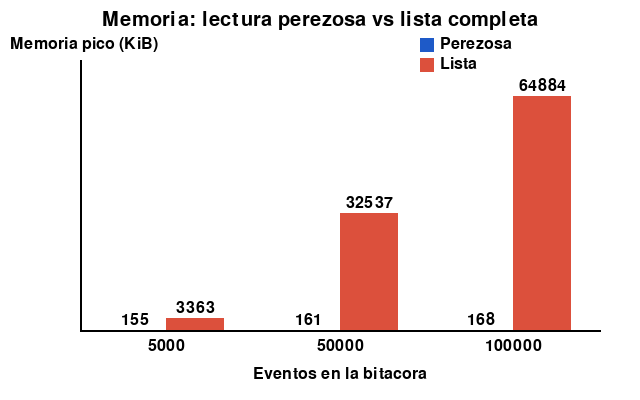
\includegraphics[width=\columnwidth]{resultados/figura_C.png}
\caption{Experimento C: memoria pico de la lectura perezosa frente a la carga completa en una lista.}
\label{fig:C}
\end{figure}

El Experimento C (Fig.~\ref{fig:C}) muestra el contraste de memoria: la lectura perezosa pasa de 154.6 a 167.7~KiB al multiplicar los eventos por 20, mientras que la lista crece de $3\,363$ a $64\,884$~KiB, entre 665 y 690 bytes por evento. Los tiempos de ambos recorridos son parecidos; la lista salió algo más rápida en parte porque se midió después y el sistema ya tenía el archivo en caché, así que la ventaja de la lectura perezosa está en la memoria y no en el tiempo.

\section{Discusión}\label{sec:disc}
\subsection{Tamaño del buffer}
Cada aumento de 10 veces en el buffer mejora menos que el anterior: 7.5, 4.7 y 1.75 veces. Con $N=100$ se obtiene casi toda la ganancia (0.35~s frente a 12.37~s con $N=1$), y pasar a 1000 solo ahorra 0.15~s por cada $100\,000$ eventos, a cambio de arriesgar hasta 999 eventos en memoria si el juego se cierra de golpe. Por eso se eligió $N=100$. Como \texttt{flush()} entrega los datos al sistema operativo pero no garantiza que lleguen al disco, en un HDD el experimento mide sobre todo el costo de las llamadas al sistema.

\subsection{Criterios de valores atípicos}
Con los diez puntajes de referencia, la regla del IQR marca el 9000 (límites $-750$ y $5250$), pero su puntaje $z$ es 2.70 y no supera 3. La diferencia es que el valor sospechoso participa en el cálculo de la media y de la desviación: la media sube a 2850 (la mediana es 2250) y la desviación a 2281.45, lo que acerca el valor al centro. De hecho, con $n=10$ ningún dato puede superar $|z|=(n-1)/\sqrt{n}\approx 2.85$, así que el criterio $|z|>3$ no puede detectar nada. La mediana y los cuartiles son robustos porque un valor extremo no los mueve, y la media y la desviación no. Para detectar tramposos conviene la regla del IQR.

\subsection{Datos del juego}
La bitácora real tiene 25 sesiones terminadas y 1238 líneas, todas válidas: 18 sesiones terminaron en muerte y 7 por abandono voluntario (\texttt{result=quit}); 4 se jugaron en easy, 10 en hard y 11 en normal. Los abandonos se incluyen en las medidas, porque el abandono es justamente lo que mide el embudo, aunque los más cortos probablemente explican el puntaje mínimo de 0.

\emph{Distribución.} El puntaje tiene media 4616 y mediana 3200, con $CV=90.4\,\%$, la más alta de las tres variables (duración $72.6\,\%$, daño por golpe $31.4\,\%$), así que es la más inestable. Que la media supere a la mediana indica asimetría a la derecha. El histograma de 8 intervalos es bimodal: 8 sesiones caen en el primer intervalo (0 a 1662) y 6 en el de 8312 a 9975. Ningún criterio marcó atípicos: el máximo ($13\,300$) queda por debajo del límite superior del IQR ($21\,075$) y tiene $z=2.08$. Con la regla de Sturges, $k=\lceil 1+\log_2 25\rceil=6$ \cite{sturges}, los intervalos serían más anchos (unos 2217 puntos) y la forma bimodal probablemente se suavizaría, aunque no se probó.

\emph{Embudo.} De 25 sesiones, 20 llegaron al nivel 2 (abandono de $20.0\,\%$) y solo 1 llegó al nivel 10. Los mayores abandonos relativos están al final: $33.3\,\%$ en el nivel 8, $50.0\,\%$ en el 9 y $66.7\,\%$ en el 10, calculados sobre 9, 6 y 3 sesiones. En números absolutos, el nivel 1 es el que más sesiones pierde (5 de 25).

\emph{Dificultad.} En easy ($n=4$) la media es 6175 con desviación 3905; en hard ($n=10$), 4050 con 3703.5. La diferencia de 2125 puntos ($34.4\,\%$ de la media de easy) es menor que la desviación de cada grupo, así que con 4 y 10 sesiones no se puede afirmar que la dificultad afecte el puntaje.

\emph{Relación.} Duración y puntaje tienen $r=0.9853$ (muy fuerte según \cite{evans}), lo esperable porque el puntaje se acumula con el tiempo sobrevivido. El daño total de la sesión contra el nivel alcanzado da $r=0.7915$ (fuerte), lo que no significa que recibir daño ayude a avanzar: ambas variables crecen con el tiempo que el jugador sobrevive.

\emph{Cambio de diseño.} Desde el nivel 8 los drones igualan la velocidad del jugador (5), y desde el 9 los robots también y la espera entre apariciones llega a su mínimo de 30 fotogramas. Eso coincide con los abandonos de 33 a 67\,\%, aunque no se comprobó que sea la causa. Se propone limitar la velocidad de los enemigos a 4 y subir más despacio la cantidad de enemigos desde el nivel 8, y volver a medir el embudo.

\section{Conclusiones}
Se construyó un sistema de telemetría con escritura incremental, rotación, lectura en streaming tolerante a corrupción y un motor estadístico propio que reproduce exactamente los valores de referencia y se visualiza dentro del juego. La lectura perezosa mantuvo la memoria casi constante (unos 160~KiB), frente a una lista que crece con el archivo ($64\,884$~KiB con $100\,000$ eventos).

Entre las limitaciones: la mediana, los cuartiles y el P90 exigen guardar los datos, y el histograma necesita dos recorridos. La varianza calculada con suma de cuadrados puede perder precisión con valores muy grandes, y el método de Welford \cite{welford} es una alternativa más estable. Además, \texttt{flush()} no garantiza la escritura física, la dispersión dibuja solo una muestra de 500 puntos y no se escapan los delimitadores dentro de los valores. Como trabajo futuro quedan el escape de delimitadores, un estimador de la mediana sin guardar los datos y un formato con versión de esquema.

\begin{thebibliography}{1}
\bibitem{drachen} A. Drachen, M. Seif El-Nasr, and A. Canossa, ``Game analytics---The basics,'' in \emph{Game Analytics: Maximizing the Value of Player Data}, M. Seif El-Nasr, A. Drachen, and A. Canossa, Eds. London, U.K.: Springer, 2013.
\bibitem{tukey} J. W. Tukey, \emph{Exploratory Data Analysis}. Reading, MA, USA: Addison-Wesley, 1977.
\bibitem{hyndman} R. J. Hyndman and Y. Fan, ``Sample quantiles in statistical packages,'' \emph{Amer. Statist.}, vol. 50, no. 4, pp. 361--365, 1996.
\bibitem{welford} B. P. Welford, ``Note on a method for calculating corrected sums of squares and products,'' \emph{Technometrics}, vol. 4, no. 3, pp. 419--420, 1962.
\bibitem{sturges} H. A. Sturges, ``The choice of a class interval,'' \emph{J. Amer. Statist. Assoc.}, vol. 21, no. 153, pp. 65--66, 1926.
\bibitem{evans} J. D. Evans, \emph{Straightforward Statistics for the Behavioral Sciences}. Pacific Grove, CA, USA: Brooks/Cole, 1996.
\bibitem{tracemalloc} Python Software Foundation, ``tracemalloc---Trace memory allocations,'' \emph{Python 3 Documentation}. [Online]. Available: \url{https://docs.python.org/3/library/tracemalloc.html}
\end{thebibliography}

\end{document}
